\documentclass[border=6pt]{standalone}
% Shared preamble of every figure (included by each fig*.tex)
\usepackage{fontspec}
\setmainfont{DejaVu Sans}
\setmonofont{DejaVu Sans Mono}
\usepackage{amsmath,amssymb}
\usepackage{tikz}
\usetikzlibrary{positioning,arrows.meta,fit,calc,decorations.pathreplacing,shapes.geometric,backgrounds}
\definecolor{cdata}{HTML}{4C78A8}
\definecolor{cmodel}{HTML}{F58518}
\definecolor{chead}{HTML}{54A24B}
\definecolor{cgold}{HTML}{E45756}
\definecolor{cgrey}{HTML}{9D9D9D}
\definecolor{cfull}{HTML}{B279A2}
\tikzset{
  box/.style={draw, rounded corners=2pt, align=center, inner sep=4pt, font=\small, minimum height=8mm},
  data/.style={box, fill=cdata!15, draw=cdata!80!black},
  model/.style={box, fill=cmodel!18, draw=cmodel!80!black},
  head/.style={box, fill=chead!18, draw=chead!70!black},
  note/.style={font=\footnotesize, align=center, text=black!70},
  arr/.style={-{Stealth[length=2.2mm]}, thick, black!70},
}

\begin{document}
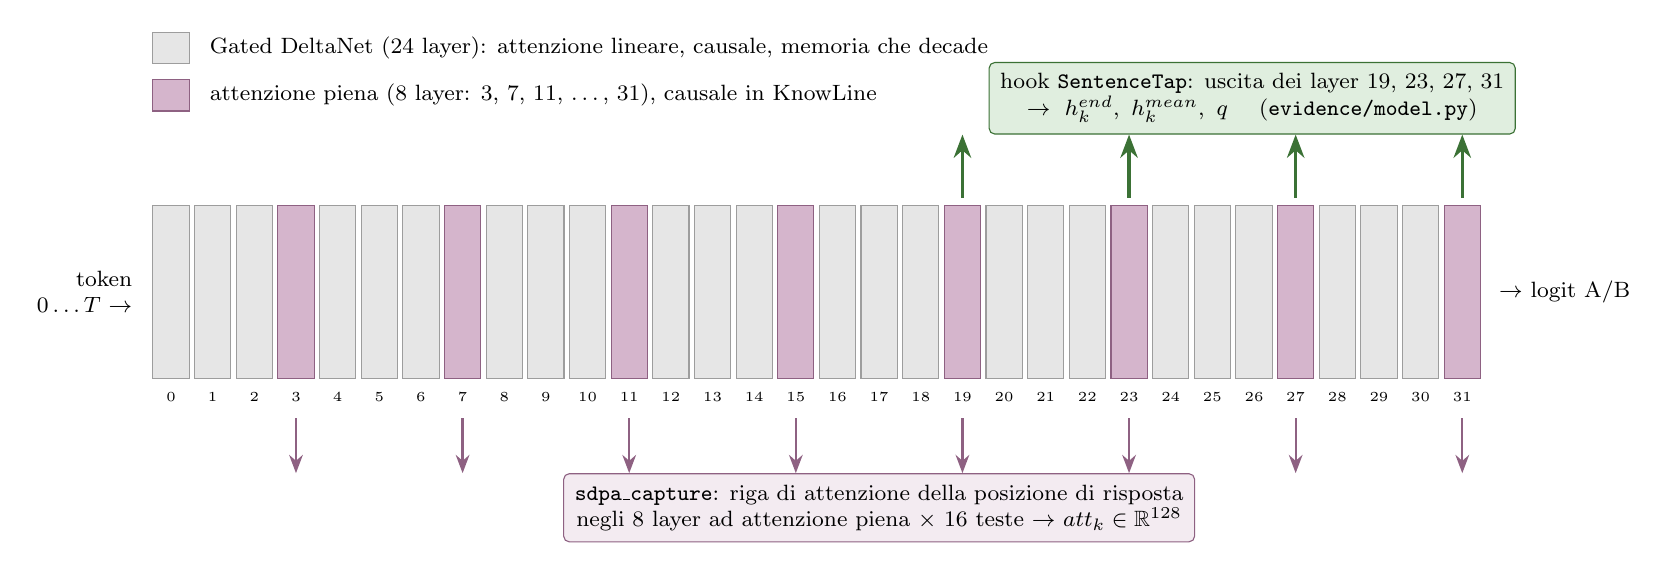
\begin{tikzpicture}[x=4.6mm,y=1mm]
% 32 layers as columns
\foreach \l in {0,...,31}{
  \pgfmathtruncatemacro{\m}{mod(\l,4)}
  \ifnum\m=3
    \fill[cfull!55, draw=cfull!80!black] (\l*1.15,0) rectangle ++(1,22);
  \else
    \fill[cgrey!25, draw=cgrey] (\l*1.15,0) rectangle ++(1,22);
  \fi
  \node[font=\tiny, anchor=north] at (\l*1.15+0.5,-0.5) {\l};
}
% read markers on 19 23 27 31
\foreach \l in {19,23,27,31}{
  \draw[chead!70!black, very thick, -{Stealth}] (\l*1.15+0.5,23) -- (\l*1.15+0.5,31);
}
\node[head, anchor=south, font=\footnotesize] at (25*1.15+1.6,31) {hook \texttt{SentenceTap}: uscita dei layer 19, 23, 27, 31\\$\to\ h^{end}_k,\ h^{mean}_k,\ q$ \quad (\texttt{evidence/model.py})};
% attention rows on all full layers
\foreach \l in {3,7,11,15,19,23,27,31}{
  \draw[cfull!80!black, thick, -{Stealth}] (\l*1.15+0.5,-5) -- (\l*1.15+0.5,-12);
}
\node[box, fill=cfull!15, draw=cfull!80!black, anchor=north, font=\footnotesize] at (17*1.15+0.5,-12) {\texttt{sdpa\_capture}: riga di attenzione della posizione di risposta\\negli 8 layer ad attenzione piena $\times$ 16 teste $\to$ $att_k \in \mathbb{R}^{128}$};
% legend
\fill[cgrey!25, draw=cgrey] (0,40) rectangle ++(1,4); \node[anchor=west,font=\footnotesize] at (1.3,42) {Gated DeltaNet (24 layer): attenzione lineare, causale, memoria che decade};
\fill[cfull!55, draw=cfull!80!black] (0,34) rectangle ++(1,4); \node[anchor=west,font=\footnotesize] at (1.3,36) {attenzione piena (8 layer: 3, 7, 11, \dots, 31), causale in KnowLine};
\node[font=\footnotesize, anchor=east, align=right] at (-0.3,11) {token\\$0 \dots T$ $\to$};
\node[font=\footnotesize, anchor=west] at (32*1.15+0.1,11) {$\to$ logit A/B};
\end{tikzpicture}
\end{document}
